\documentclass[11pt]{article}
\usepackage[margin=0.5in]{geometry}
\usepackage{amsmath}
\usepackage{amsfonts}
\usepackage{algorithm}
\usepackage{algpseudocode}
\usepackage{graphicx}
\usepackage{subcaption}
\usepackage{booktabs}
\usepackage{hyperref}
\usepackage{cite}

\title{ELEC5660 Project 1 Phase 2 Report}
\author{SIT, IOK LONG}
\date{\today}

\begin{document}
\maketitle

\section{Introduction}

This report presents the implementation of the A* (A-Star) path planning algorithm for 3D grid-based navigation. The algorithm plans collision-free paths in a three-dimensional environment with obstacles.

\section{A* Implementation Details}

\subsection{State Representation}

Each state in our A* implementation is represented as a 3D grid coordinate:
\begin{equation}
    s = (x, y, z) \quad \text{where} \quad x, y, z \in \mathbb{Z}
\end{equation}

The grid uses 1-based indexing with bounds:
\begin{equation}
    1 \leq x \leq \text{max}_x, \quad 1 \leq y \leq \text{max}_y, \quad 1 \leq z \leq \text{max}_z
\end{equation}

For visualization and execution, grid indices are converted to cell-center coordinates:
\begin{equation}
    p_{\text{world}} = [x - 0.5, y - 0.5, z - 0.5]
\end{equation}

\subsection{Neighbor Expansion}

We use 6-connected connectivity for neighbor expansion, allowing movement along the three principal axes:
\begin{equation}
    \mathcal{N}(s) = \{s + \delta \mid \delta \in \Delta\}
\end{equation}
where
\begin{equation}
    \Delta = \{
    (\pm 1, 0, 0), 
    (0, \pm 1, 0), 
    (0, 0, \pm 1)
    \}
\end{equation}

\subsection{Heuristic Function}

We employ the Manhattan distance as our heuristic function, which is admissible and consistent for 6-connected grids:
\begin{equation}
    h(s_1, s_2) = |x_1 - x_2| + |y_1 - y_2| + |z_1 - z_2|
\end{equation}

\subsection{Cost Function}

The total cost function follows the standard A* formulation:
\begin{equation}
    f(s) = g(s) + h(s)
\end{equation}
where:
\begin{itemize}
    \item $g(s)$: Actual cost from start to state $s$ (number of steps)
    \item $h(s)$: Heuristic estimate from $s$ to goal
\end{itemize}

\section{Statistics}
\begin{figure}[htbp]
\centering
\begin{subfigure}[b]{0.32\textwidth}
    \centering
    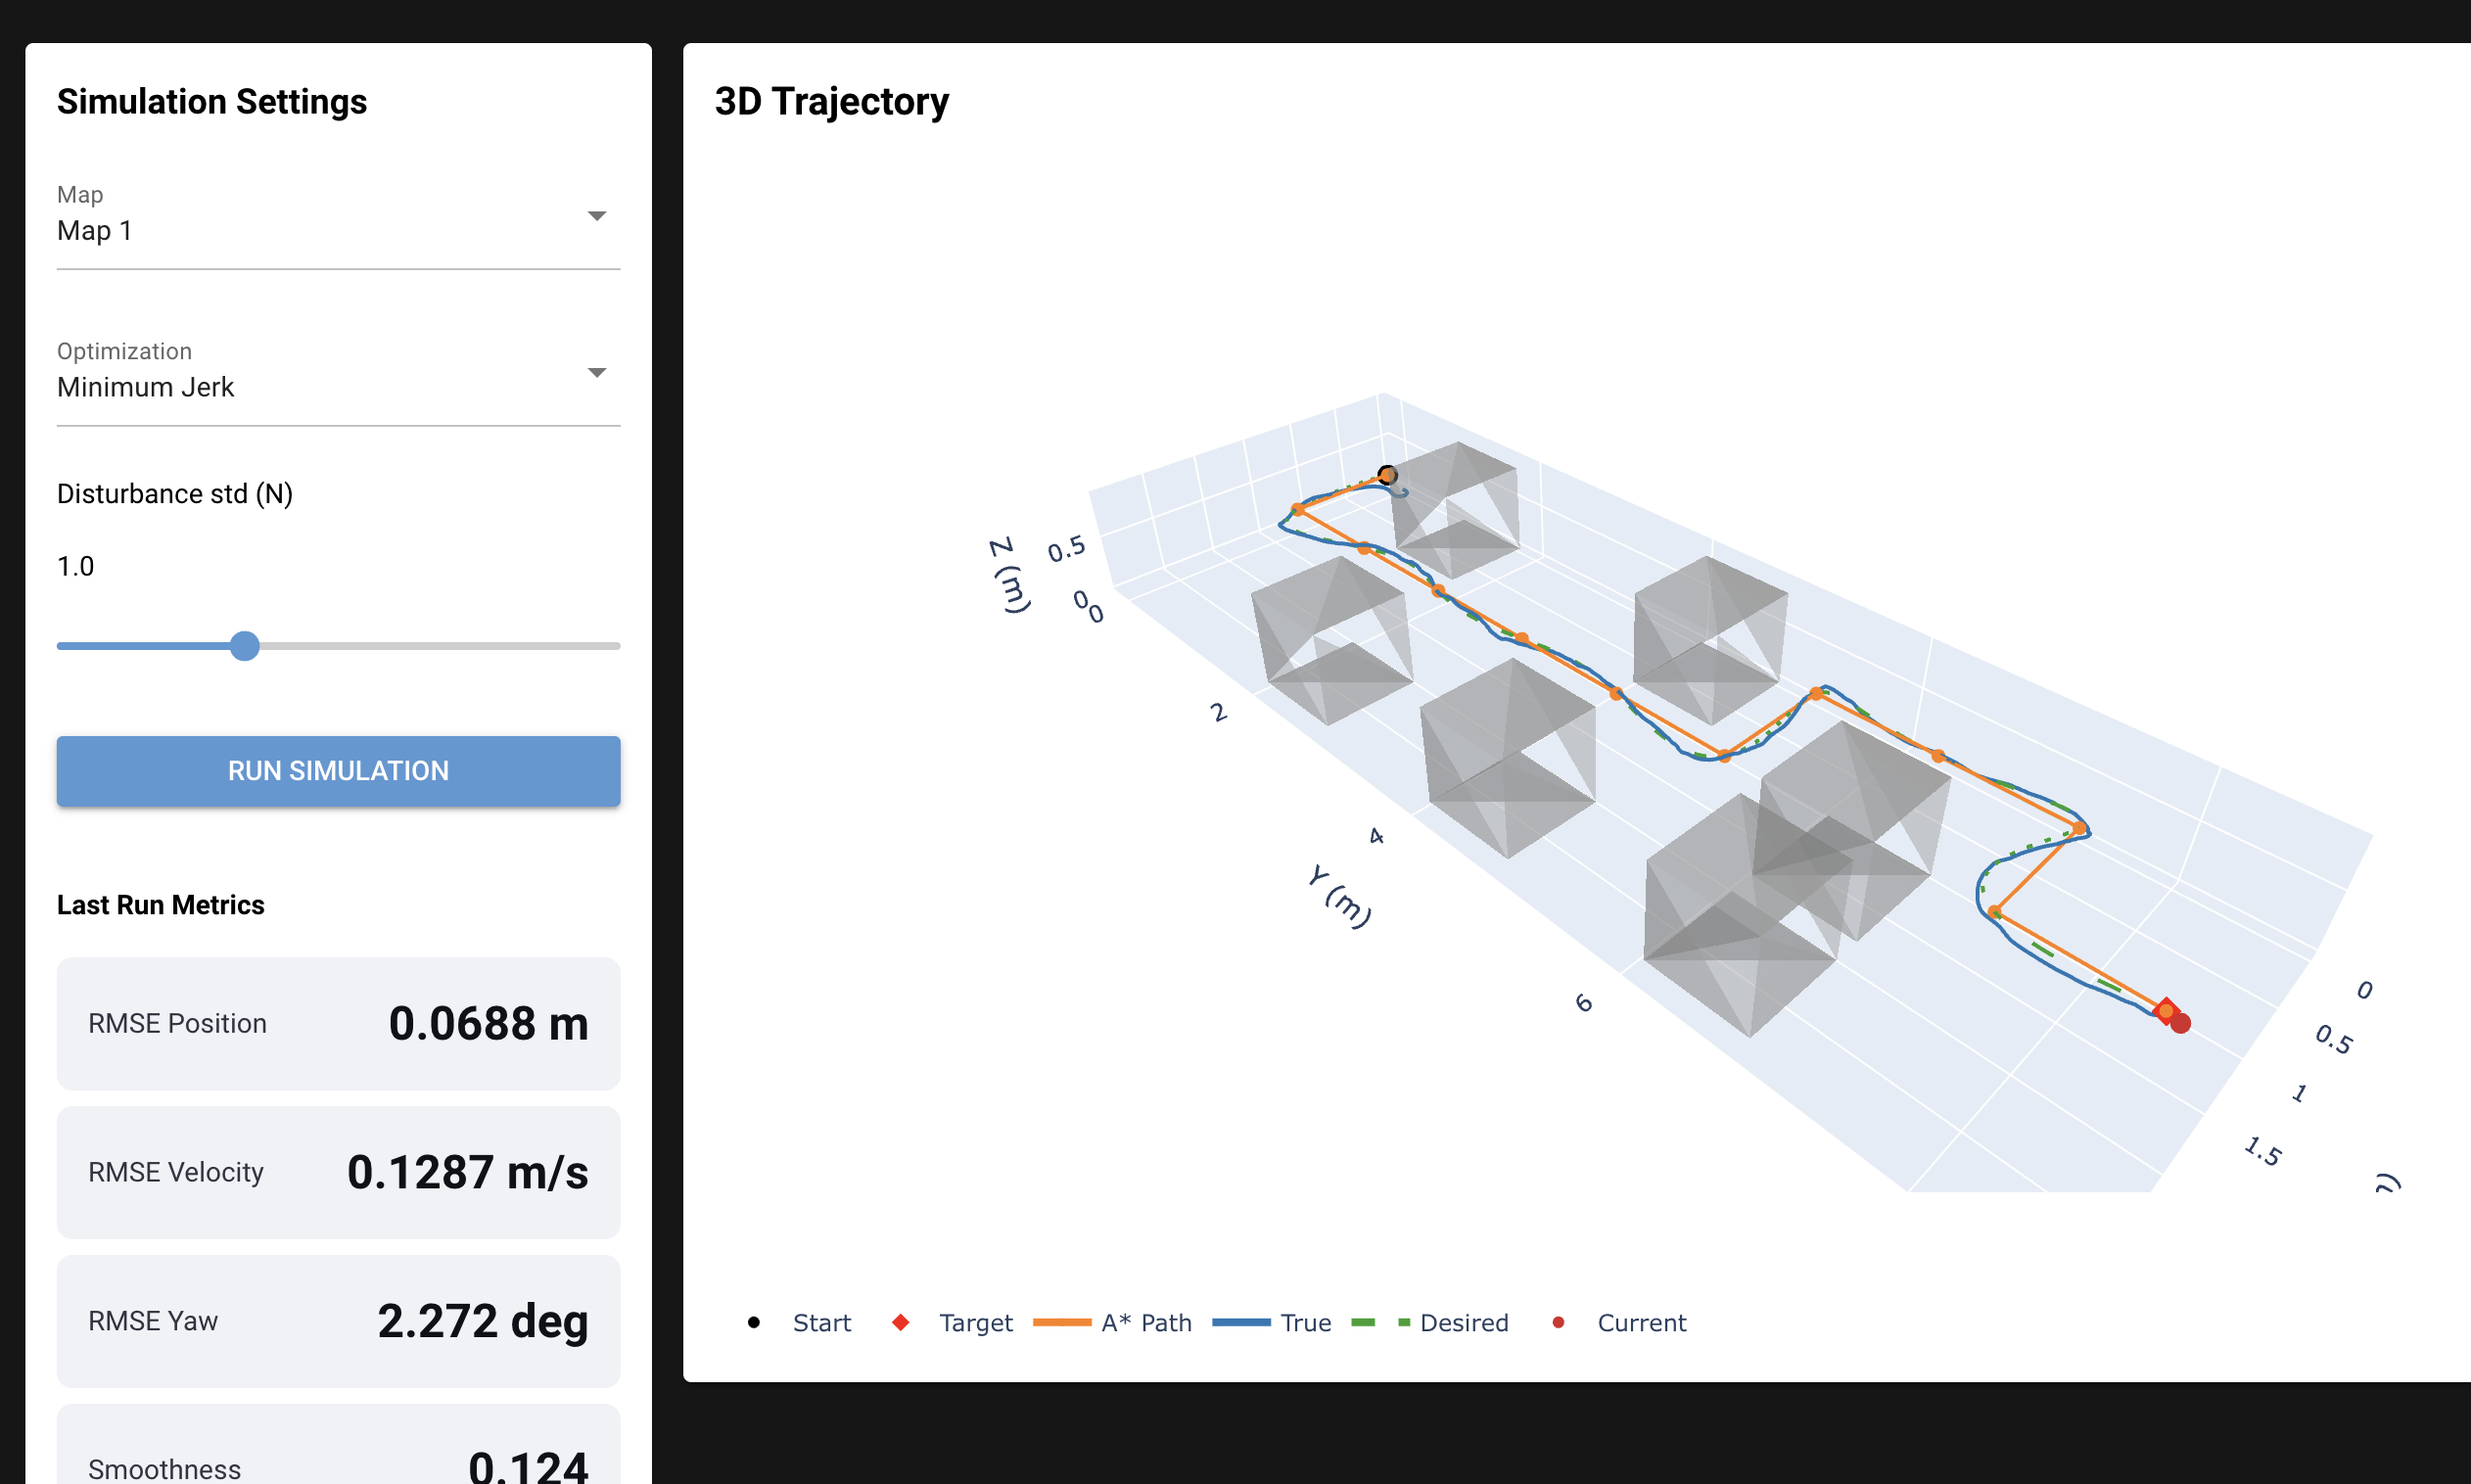
\includegraphics[width=\textwidth]{figures/map1_path.png}
    \caption{Planned path and trajectory for Map 1}
    \label{fig:map1}
\end{subfigure}\hfill
\begin{subfigure}[b]{0.32\textwidth}
    \centering
    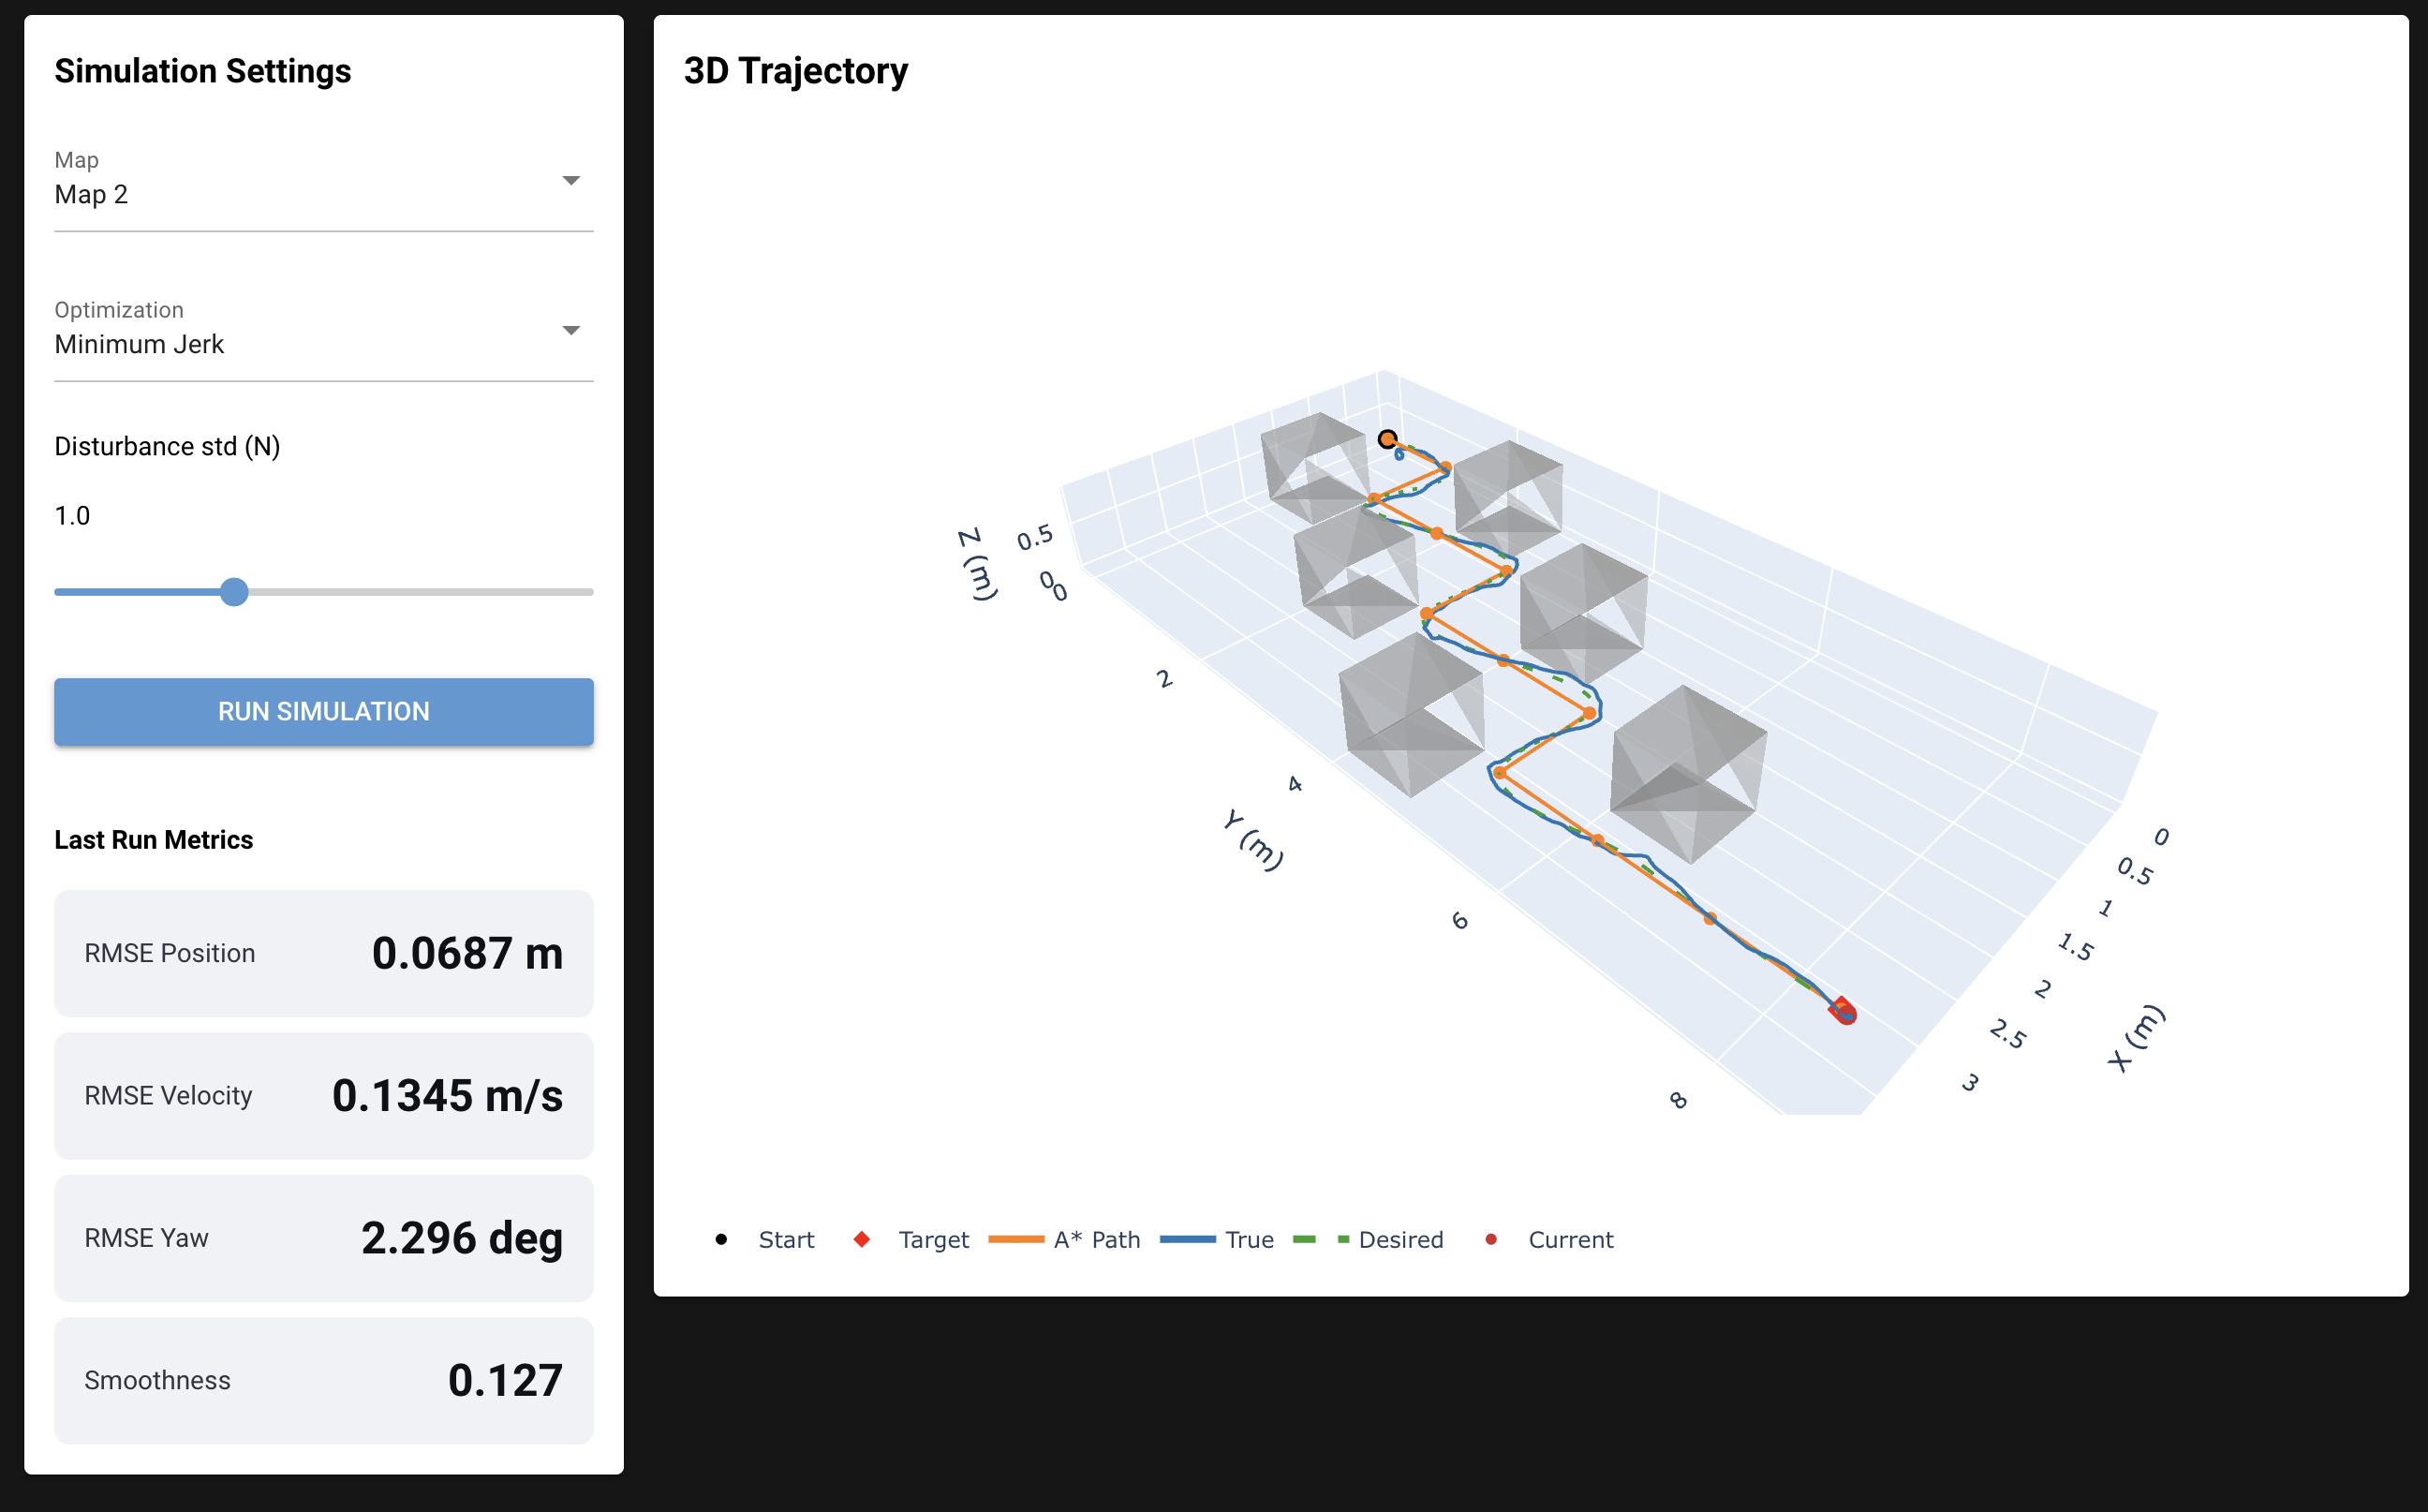
\includegraphics[width=\textwidth]{figures/map2_path.png}
    \caption{Planned path and trajectory for Map 2}
    \label{fig:map2}
\end{subfigure}\hfill
\begin{subfigure}[b]{0.32\textwidth}
    \centering
    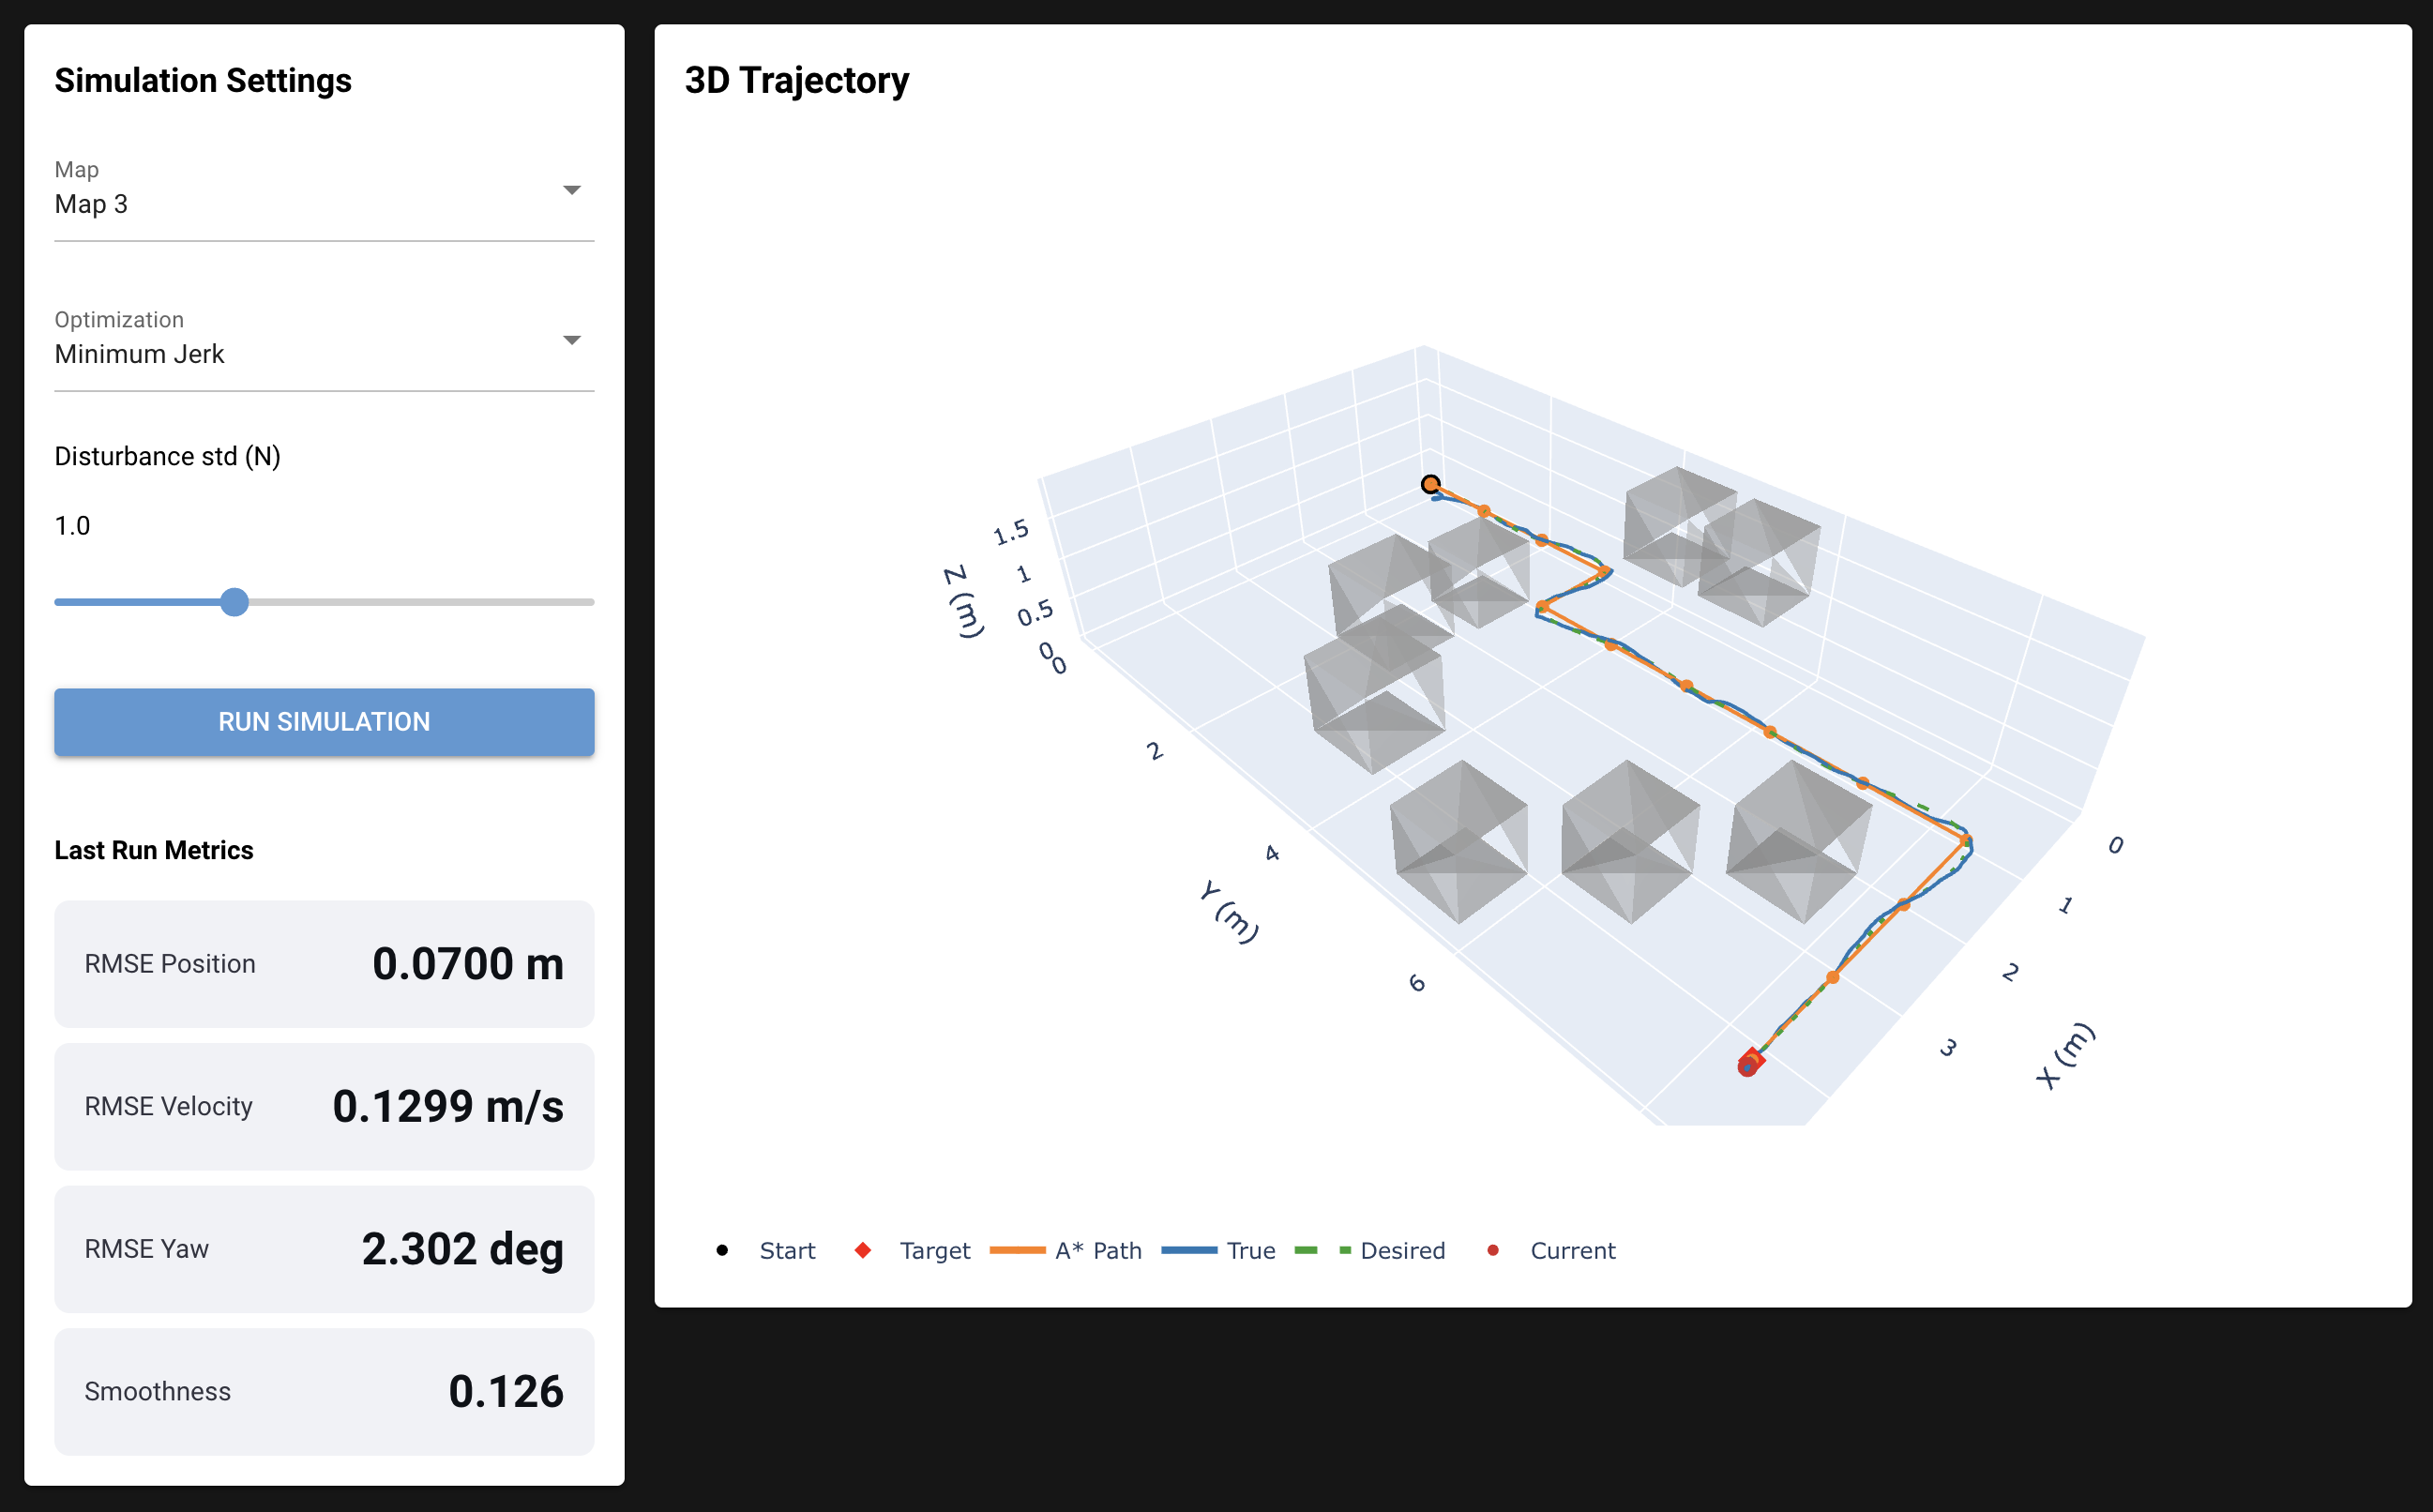
\includegraphics[width=\textwidth]{figures/map3_path.png}
    \caption{Planned path and trajectory for Map 3}
    \label{fig:map3}
\end{subfigure}
\caption{Planned paths and trajectories for Maps 1--3}
\label{fig:maps_row}
\end{figure}

\begin{table}[htbp]
\centering
\caption{Path Planning Statistics}
\label{tab:stats}
\begin{tabular}{lccc}
\toprule
\textbf{Metric} & \textbf{Map 1} & \textbf{Map 2} & \textbf{Map 3} \\
\midrule
RMSE Position (m) & 0.0688 & 0.0687 & 0.0700 \\
RMSE Velocity (m/s) & 0.1287 & 0.1345 & 0.1299 \\
RMSE Yaw (rad) & 0.03965 & 0.04007 & 0.04018 \\
Smoothness Score & 0.124 & 0.127 & 0.126 \\
\bottomrule
\end{tabular}
\end{table}
\end{document}